% !TeX spellcheck = en_US
\chapter{Introduction}
\label{chap:intro}

Wind energy is widely becoming recognized as one of the most cost efficient renewable energy sources.
It is predicted that by the end of 2014 the worlds wind energy production will reach 360GW~\cite{worldwidewindcapacity}.
Heavyweight energy consumer USA has declared a goal of reaching 20\% wind energy of the total energy consumed in 2030~\cite{20percentenergy}, the European Union has committed to a similar goal of 20\% renewable energy by 2020~\cite{directive2009}.

Siemens Wind Power is one of the worlds leading producers of wind turbines, with a global market share of 9.5\% in 2012~\cite{worldmarketupdate2012}.
Siemens Wind Power is increasingly focusing on the offshore wind farm market.
The current setup of a wind farm requires additional infrastructure for management of the wind farm.
As well as the wind turbines the wind farm consists of a SCADA system for operations that involve the entire farm, such as external requests, and multiple park regulators, for near realtime control of the turbines.
The SCADA system and the park pilots are centralized control points of the wind farm. Having centralized control means that the system has single points of failure, which if it fails decreases the availability of the wind farm.
Furthermore the SCADA system and park regulators does not scale automatically with the number of turbines, but needs hardware to be upgraded if too many turbines are added.

Since wind energy is recognized as one of the solutions to the renewable energy problem, wind park size and capacity keeps increasing.
The need for scalability is thus not only a challenge for Siemens Wind Power but for the entire industry.

Despite the fact that the wind farms has grown to a size that is becoming increasingly hard to manage with a centralized control system the area of decentralization in wind farm management and control has largely been neglected as a research area. The main problem being that with a centralized control system individual turbines must wait for the centralized control system to calculate and communicate values like the amount of power a single turbine must produce in order to meet the power production requirements of the entire wind farm. Since the wind farm is expected to operate as a single unit the power production of a single turbine is affected by the power production of all other turbines. This interdependence between all turbines forces the central control system to collect data from all turbines before a single new power production value can be calculated, which is time consuming. Adding turbines will additionally increase the time the centralized control system needs to calculate new power production values. To uphold a constant power production level for the entire wind farm near real-time control and regulation is necessary thus the time consumption of the centralized control system must be minimized in effect limiting the number of turbines the centralized control system is able to handle.

\section{Siemens Wind Power case}

% Beskriv topologi
% Regulerings algoritmen tager kun 30 ms. 150 ms er cycle time

\label{sec:SiemensCase}
Siemens Wind Power builds wind farms of different sizes ranging from single turbines to well above one hundred turbines. \cite{simensOffShoreProjects, simensOnShoreProjects}.

Today turbines in a wind farm at Siemens are equipped with computers for the purpose of regulating power production parameters, data collection and for communication with the rest of the system. The current wind farm setup is illustrated on \cref{fig:currentSiemensSetup}. Every turbine is connected to a Wind Power Supervisor, which is a central component that aggregates data, stores data and handles wind park communication with the outside world. At Siemens up to eight Park Pilots are present pr. wind farm and one Wind Power Supervisor.

\begin{figure}
	\centering
	\scalebox{0.7}{\tikzstyle{line} = [draw, -latex']

\begin{tikzpicture}
[
	start chain=going right,
	diagram item/.style={
		minimum width=40pt,
		on chain,
	},
	mill item/.style={
			minimum width=10pt,
			on chain
	},
	comment item/.style={
			inner sep=5pt,
			draw,
			dashed,
	}
]

\newcommand\millFigure{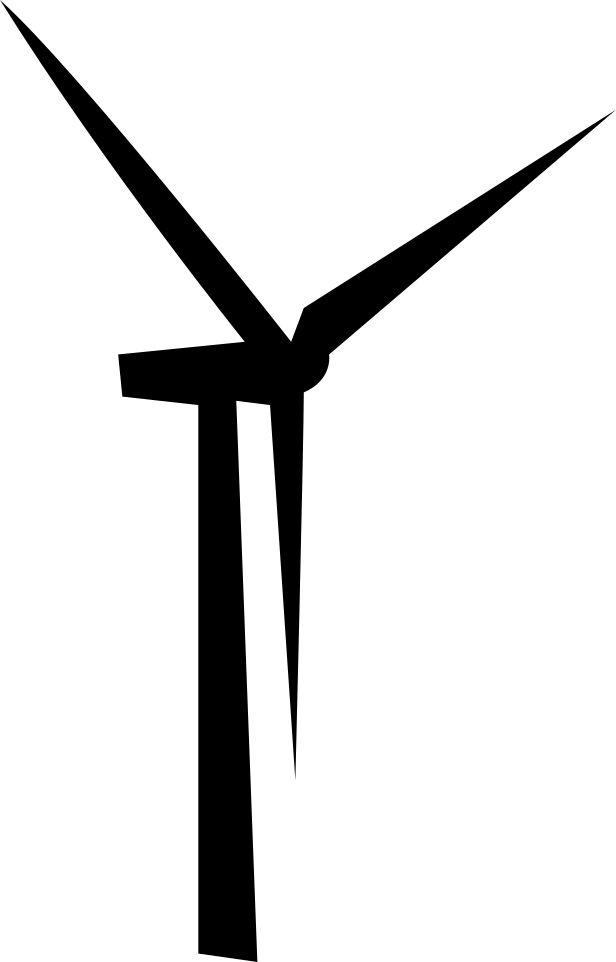
\includegraphics[width=0.7cm]{MillSiluet}}
\newcommand\multiMillFigure{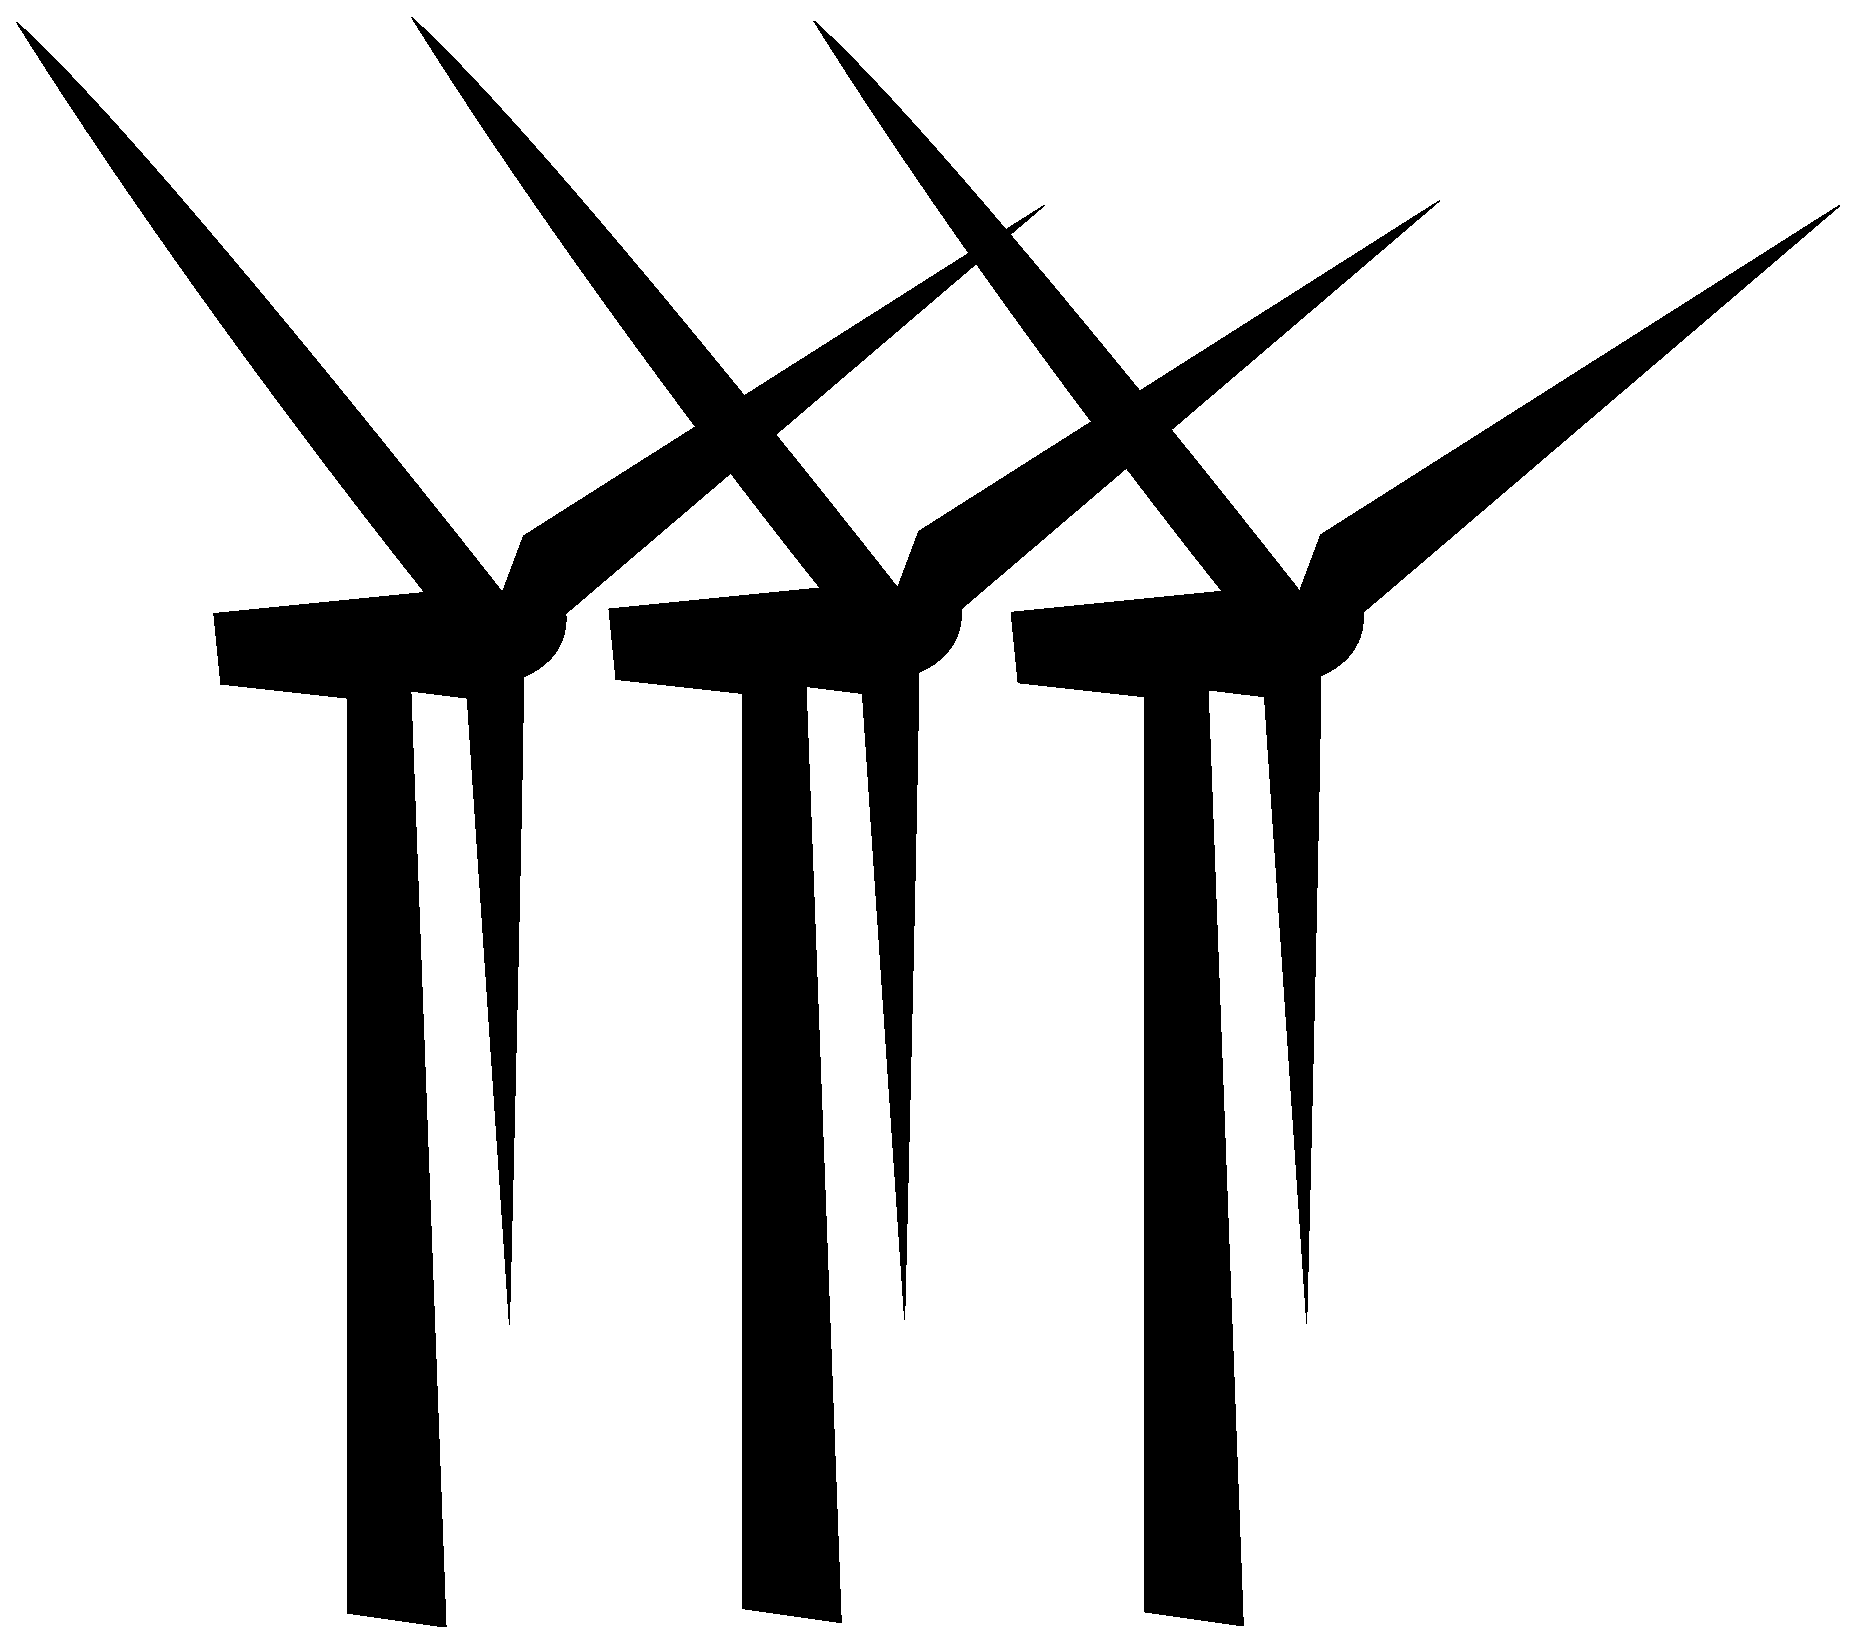
\includegraphics[width=4cm]{MultiMillSiluet}}

\begin{scope}[node distance=20mm and 10mm]

\node [
	diagram item,
	label=center:Internet
] (Internet) {\includegraphics[width=4cm]{Cisco_BW/cloud}};

\node [
	continue chain=going below,
	diagram item,
	label={[label distance=0cm]80:Wind Power Supervisor}
] (wps){\includegraphics[width=1.5cm]{Cisco_BW/fileserver}};

\node [
	start branch=1 going left,
	diagram item,
	label=above:High Performance Park Pilot
] (hppp){\includegraphics[width=1.5cm]{Cisco_BW/fileserver}};

\node[
	comment item,
	align=left
](comment)[right=4cm of wps]{
	\begin{tabular}{l}
		\textbf{Wind Power Supervisor}  \\
		Control tasks\\
		- Noise control \\
		- Flicker control \\
		- Aviation light control \\
		- Ice control \\
		Data \\
		- Aggregated historical \\
		- Reporting \\
		External communication \\
		- Network services \\
	\end{tabular}
};

\node [	
continue chain=going below,
mill item
] (millright){\multiMillFigure};

\node[
	comment item,
	align=left
](comment1)[right=3.0cm of millright]{
Each turbine contains logged \\
data with high resolution and \\
turbine control logic.};

\node [	
continue branch=1 going below,
mill item
] (millleft){\multiMillFigure};

\draw [->] (hppp.251) -- (millleft.101) node [near start, left] {1} node [midway] (hiddenNode){};

\node[
	comment item,
	align=left
](comment2)[left=1.7cm of hiddenNode]{
HPPP \\
getCurrentStatus() \\
calculateSetpoints() \\
setNewSetpoints() };

\path [line,dashed] (wps) -- (comment);
\path [line,dashed] (millright) -- (comment1);
\path [line,dashed] (hiddenNode) -- (comment2);

\draw [->] (hppp.280) -- (millleft.84) node [near end, right] {*};
\draw [<-] (hppp.265) -- (millleft.93);

\draw (Internet) -- (wps);
\draw (wps) -- (hppp) node [near start, above] {1} node [near end, below] {*};
\draw (wps) -- (millright) node [near start, left] {1} node [near end, right] {*};

\end{scope}

\end{tikzpicture}}
	\captionsetup{format=plain,font=footnotesize,labelfont={bf,defaultCapFont},labelsep=quad,singlelinecheck=no}
	\caption[The current Siemens wind farm system overview]{
		\label{fig:currentSiemensSetup} 
		\footnotesize{%
			The current Siemens system overview.
		}
	}
\end{figure}

For every transformer station there is a Park Pilot. The Park Pilots are responsible for wind farm regulation. This is done by monitoring all the turbines performance parameters and issuing setpoints for power production. The calculation of setpoints for each turbine consist of a number of steps as illustrated on figure \cref{fig:currentSiemensCycleTime}. First the Park Pilot must request data from each turbine in order to calculate setpoints based on updated values. The Park Pilot must wait for each turbine to answer the request. After receiving data from each turbine new setpoints are calculated and distributed to the turbines. The buffer is added to make sure setpoints has been properly distributed and that individual turbines have time to adjust their power production according to the new setpoint before a new request for turbine data is sent. Also the WaitForData block may vary in time depending on the current traffic of the network as well as the response time of the individual turbines.

\begin{figure}[!h]
	\centering
	\input{figures/tikz/timingDiagramSiemensSystem}
	\captionsetup{format=plain,font=footnotesize,labelfont={bf,defaultCapFont},labelsep=quad,singlelinecheck=no}
	\caption[The current Siemens wind farm system overview]{
		\label{fig:currentSiemensCycleTime} 
		\footnotesize{%
			The regulation cycle.
		}
	}
\end{figure}

Every turbine has a database for data logging purposes, this database is replicated to the Wind Power Supervisor.
The Wind Power Supervisor does data aggregation on data from each turbine as well as store a copy of the replicated data.
The turbines, Wind Power Supervisor and Park Pilots are connected with a gigabit network, which currently has plenty of extra capacity in terms of available bandwidth.
The system handles more than 50 control points and 200 measurement points and samples these every 50 ms.

%\begin{figure}
%	\centering
%	\begin{sequencediagram} %Created using pgf-umlsd
%		\newthread{reg}{:Park Pilot}
%		\newinst[2]{turbine}{:Turbine}
%	
%		\begin{sdblock}{each turbine}{}
%			\mess[1]{reg}{getCurrentStatus}{turbine}
%			\mess[1]{turbine}{status}{reg}
%		\end{sdblock}
%		
%		\begin{call}{reg}{calculateAllSetpoints()}{reg}{}
%		\end{call}
%	
%		\begin{sdblock}{each turbine}{}
%			\mess[1]{reg}{setNewSetpoint}{turbine}
%		\end{sdblock}
%					
%	\end{sequencediagram}
%
%	\captionsetup{format=plain,font=footnotesize,labelfont={bf,defaultCapFont},labelsep=quad,singlelinecheck=no}
%	\caption[Regulator calculation sequence]{
%		\label{fig:dataComputationSequence} 
%		\footnotesize{%
%			Regulator calculation sequence.
%		}
%	}
%\end{figure}

\section{Thesis motivation}
\label{sec:ThesisMotivation}
Todays setup at Siemens Wind Power (\cref{sec:SiemensCase}) is an example of a system wished to be made less centralized. The current setup poses the following challenges to Siemens:  

\begin{itemize} 
	\item Single point of failure. Should a Wind Power Supervisor or a Park Pilot fail, a part of the wind farm will become unavailable.
	\item Low scalability. The Wind Power Supervisors and Park Pilots does not scale with the number of turbines. This is reflected in the wind farm regulation performance. Today a wind farm regulation cycle time is 150 ms. This regulation cycle time is set after worst case setpoint retrieval time, worst case new setpoint calculations and worst case time it takes to broadcast new setpoints. This ultimately depends on worst case number of turbines pr. Park Pilot.
\end{itemize}

Siemens wishes to decentralize the Wind Power Supervisor and Park Pilots by distributing their functionality to the turbines, utilizing the free computing capacity of the computers already residing in every turbine. This would increase availability by lowering the possibility of single point of failure. Furthermore this would increase scalability of the system, opening for performance optimizations of the wind farm regulation cycle time by detaching regulation time from the number of turbines pr. Park Pilot. 

\section{Problem statement}
\label{sec:problemStatement}

The purpose of this thesis is to design, implement and evaluate a solution for a Siemens wind farm, where the Wind Park Supervisor and the Park Pilots are decentralized by utilizing the free capacity residing in every turbine for the Siemens Wind Power case. The solution must be able to provide the same features as the current wind farm setup. 

\paragraph{The following problems are addressed:}
\begin{description} % [label={\arabic*.}, ref=\textit{\arabic*}]
	%	\label{PS:Q:1}
	\labitem{Feasibility}{PS:Q:Feasibility} How can we best re-implement the current Siemens system (\cref{sec:SiemensCase}) as a system where the Wind Park Supervisor and the Park Pilots are decentralized?
	%	\label{PS:Q:4}
	\labitem{Availability}{PS:Q:Availability} Can we create a solution where removing one or more nodes from the system at runtime does not cause system failure?
	%	\label{PS:Q:3}
	\labitem{Performance}{PS:Q:Performance} Can we create a solution that scales so the number of turbines does not impact the regulation cycle time?
	%	\item Can we, with the new decentralized solution, reduce the current regulation cycle time of 150 ms?
	%	\label{PS:Q:2}
	\labitem{Scalability}{PS:Q:Scalability} How will the new decentralized solution influence the following parameters compared to the current Siemens system:
	\begin{enumerate}
		\item Time in milliseconds of a single regulation cycle.
		\item Network traffic measured in bits per second.
		\item Memory impact measured in bytes.
	\end{enumerate}
\end{description}

The decentralized solution will be implemented as a prototype, for proof of concept and test purposes.

\section{Enabling comparison of current Siemens system with decentralized solution} %
\todo{Bad Section title}
In order to address the problems presented in \cref{sec:problemStatement} a common ground must be established for comparison purposes. The decentralized solution proposed in this thesis will not be directly comparable to the current Siemens system because we are unable to duplicate the environment of the current Siemens system. As a consequence of this a centralized solution resembling the current Siemens system must be developed to enable a comparison. As presented in \cref{fig:projectDiffOverview} there exist a difference between the current Siemens system and the centralized solution as well as a difference between the centralized solution and the decentralized solution, illustrated by deltas.\todo{Rename figure parts. Siemens -> Current Siemens system, Central -> Centralized solution, Decentralized -> Decentralized solution}

\begin{figure}[!h]
	\centering
	\begin{tikzpicture}[
	node distance = 0.3cm,
	auto,
	block/.style={draw, rectangle, text width=5em, text centered, minimum height=5cm}		
	]
% Place nodes
\node [block]			(Siemens)												[label=above:Siemens system]	{};
\node []					(SimCen)		[right = of Siemens] 	{$\Delta$};
\node [block]			(OurCent)		[right = of SimCen] 	[label=above:Centralized solution]	{};

\begin{scope}[on background layer]
\node [block] 		(Central) 	[fit=(Siemens) (OurCent), inner sep=20pt] {};
\node []					(CenDece)		[right = of Central] 	{$\Delta$};
\node [block]			(DeCent)		[right = of CenDece] 	[label=above:Decentralized solution] {};
\end{scope}

\end{tikzpicture}
	\captionsetup{format=plain,font=footnotesize,labelfont={bf,defaultCapFont},labelsep=quad,singlelinecheck=no}
	\caption[Comparison overview]{
		\label{fig:projectDiffOverview} 
		\footnotesize{%
			Comparison overview.
		}
	}
\end{figure}

The delta between the current Siemens system and the centralized solution is minimized as much as possible based on information about the current Siemens system delivered by Siemens Wind Power. Since the operation and regulation of the current Siemens system is proprietary the full system information is not available. To make up for the missing information a number of assumptions has been done about the current Siemens system which is also a part of the delta. These assumptions will be detailed further in \cref{cha:existingSystem}. 

The delta between the centralized solution and decentralized solution describes the difference in operation of a centralized system and a decentralized system.

%ASK SIEMENS HOW TO COMPARE AND MORE CONSTRAINTS??? 

%The purpose of this thesis is to design, implement and evaluate a distributed system solution for the Siemens Wind Power case. The solution must be able to provide the same features as the current solution. The goal of the new solution is to improve scalability, availability and performance by distributing the Park Pilot and the Wind Power Supervisor onto the turbines and thereby eliminate single point of failures and make performance scale with the amount of turbines within the wind farm. 

%To realize this the system must be redesigned as a distributed system. The solution must be able to handle external requests, communication between the nodes and distribution of data, according to the Siemens case. Furthermore the solution must have a single interface for control of, and interaction with, all the nodes, in order to maintain the illusion of the wind farm serving as a single system. This means ease of access must be maintained even though computation and data is distributed among nodes. Traffic must be routed to a turbine controllers with free capacity through a single interface, without external systems being aware of it.

%This roughly leaves three essential components: A component that handles distribution of data, a component that handles communication between nodes and a load balancer, to keep track of available resources on each node. The aim to investigate, analyze and evaluate state of the art technologies within each component area and choose the technologies best suited for the Siemens case. The technologies will be weighed in terms of features with regards to the Siemens case and performance.
%
%Furthermore we aim to develop a prototype, which runs the developed solution, for proof of concept purposes. The prototype will be compared to the existing Siemens solution with respect to performance, availability and redundancy. ASK SIEMENS HOW TO COMPARE AND MORE CONSTRAINTS??? 
%
%The Siemens case presents the following constraints to the project:
%\begin{itemize}
%	\item CPU power. Our solution must be able to run on a standard consumer hardware.
%	\item Network bandwidth. Siemens uses gigabit network.
%	\item Topology. Siemens wind farms uses ring and star topology.
%\end{itemize}



% % The below snippet might come handy later on % % %
% % % % % % % % % % % % % % % % % % % % % % % % % % %
%A distributed system is a network of hardware or software components, which communicates and coordinate their actions only by message passing\cite{coulouris2005distributed}, as illustrated on \cref{fig:distributedSystem}. Each component have their own local memory every component and interact with each other in order to achieve a common goal. The nodes can be physically close, connected via a local network, or geographically distant, connected by a wide area network. An important goal of a distributed system is location transparency\cite{coulouris2005distributed} to create the illusion of the entire system acting as a single computer even though it is comprised of several nodes. Examples of distributed systems vary from aircraft control systems to the Internet to massively multiplayer online games. 
% Er det bare mig eller er det lidt rigeligt at sige at systemet agere som en enkelt computer? Lad hellere sige noget om at opnå et fælles mål? Multiplayer spil er vel ikke distribuerede systemer, men mere server client systemer.

%\begin{figure}
%	\centering
%	\includegraphics[width=0.7\textwidth,natwidth=510,natheight=542]{DistributedSystem.jpg} 
%	\captionsetup{format=plain,font=footnotesize,labelfont={bf,defaultCapFont},labelsep=quad,singlelinecheck=no}
%	\caption[Distributed Computing System with 2 nodes]{
%		\label{fig:distributedSystem} 
%		\footnotesize{%
%			A distributed system with 4 nodes.
%		}
%	}
%\end{figure}

%Distributed systems offer many benefits over centralized systems including the following\cite{IBM2005TXSeries}:
%\begin{itemize}
%	\item Scalability: It is easy to add nodes to the system, should the size of the system increase.
%	\item Redundancy: Several nodes can provide the same service, so if a node crashes, there are many to replace it. Additionally, from a cost perspective, each node does not have to be expensive, because many smaller nodes can be used as replacement.
%\end{itemize}
% Vi burde nok også snakke om ulemper? Og det er vel bare ting som er mulige at opnå?

